% Uncomment for shell escape
% \RequirePackage{shellesc}

\documentclass{article}

% Font
\usepackage{mlmodern}

% Margins
\usepackage[margin=1in]{geometry}

% Math symbols, proof environments
\usepackage{amsmath, amsthm, amssymb}

% Use this package for matrices
\usepackage{array}

% Images and positioning
\usepackage{graphicx, float, tikz}

% Trees
\usepackage{forest}

% Plots
\usepackage{pgfplots}

\usepackage{xcolor}

\usepackage{parskip}
\usepackage[T1]{fontenc}

% Math commands
\newcommand{\R}{\mathbb{R}} % Real numbers
\newcommand{\Z}{\mathbb{Z}} % Integers
\newcommand{\C}{\mathbb{C}} % Complex numbers
\newcommand{\Pow}{\mathcal{P}}
\newcommand{\set}[1]{\left\{ #1 \right\}}
\newcommand{\setc}[2]{\left\{ #1 \middle| #2 \right\}}
\newcommand{\abs}[1]{\left| #1 \right|}
\newcommand{\var}{\mathrm{VAR}}
\newcommand{\ut}[1]{\text{ #1}}
\newcommand{\cov}{\mathrm{COV}}
\newcommand{\intR}{\int_{-\infty}^{\infty}}
\newcommand{\red}[1]{\textcolor{red}{#1}}
\newcommand{\blu}[1]{\textcolor{blue}{#1}}
\newcommand{\grn}[1]{\textcolor{green}{#1}}
\newcommand{\contradiction}{\Rightarrow\!\Leftarrow}
\newcommand{\fun}{\mathrm{Fun}}

\DeclareMathOperator{\pMat}{Mat}
\newcommand{\Mat}[2]{\pMat_{#1 \times #2}}
\DeclareMathOperator{\spn}{span}
\DeclareMathOperator{\im}{im}
\DeclareMathOperator{\rank}{rank}
\DeclareMathOperator{\nul}{null}
\DeclareMathOperator{\tr}{tr}
\newcommand{\angles}[1]{\left \langle #1 \right \rangle}
\newcommand{\conj}[1]{\overline{#1}}

\title{Math 168 Homework 2}

\author{Jason Cheng}

\date{\today}

\begin{document}

\maketitle

\subsection*{Exercise 1}

Something that I'm personally interested in is language learning (I'm currently
learning Japanese). In linguistics, sentences are broken down into syntax trees,
which could be a type of network. Also, the evolution and dissipation of words
and grammar across cultures could be modeled as a type of network, with clusters
being major families of languages.

\newpage

\subsection*{Exercise 2}

The network I picked was ``Global language network'' (2014). The network models
what languages are co-spoken in order to determine the cultural influence and
``connectivity'' of languages. It also considered things like book translations,
which were modeled with directed edges. This network would not be simple since
there can be loops.

\newpage

\subsection*{Exercise 3}

\begin{enumerate}
  \item[(a)]
  \begin{gather*}
    \begin{split}
      \det(A - \lambda I) &= \det
      \begin{pmatrix}
        2 - \lambda & -1 \\
        -1 & 2 - \lambda
      \end{pmatrix} \\
      &= (2 - \lambda)^2 - (-1)^2 \\
      &= \lambda^2 - 4\lambda + 3 \\
      &= (\lambda - 3)(\lambda - 1)
    \end{split} \\
    \boxed{\lambda_1 = 1, \lambda_2 = 3}
  \end{gather*}

  \begin{gather*}
    A - 1I =
    \begin{pmatrix}
      1 & -1 \\
      -1 & 1
    \end{pmatrix}
    \rightarrow
    \begin{pmatrix}
      1 & -1 \\
      0 & 0
    \end{pmatrix} \\
    \ker(A - 1I) = \spn \set{(1, 1)}
  \end{gather*}

  The eigenvectors associated with \( \lambda_1 = 1 \) are \( \boxed{\spn
  \set{(1, 1)}} \).

  \begin{gather*}
    A - 3I =
    \begin{pmatrix}
      -1 & -1 \\
      -1 & -1
    \end{pmatrix}
    \rightarrow
    \begin{pmatrix}
      1 & 1 \\
      0 & 0
    \end{pmatrix} \\
    \ker(A - 3I) = \spn \set{(1, -1)}
  \end{gather*}

  The eigenvectors associated with \( \lambda_2 = 3 \) are \( \boxed{\spn
  \set{(1, -1)}} \).

  \item[(b)]
  \begin{enumerate}
    \item[(i)]
    \[ Ax = \lambda x \implies (-A)x = -(Ax) = -\lambda x \]

    The eigenvalues of \( -A \) are \( -\lambda_1, -\lambda_2, \dotsc,
    -\lambda_n \).

    \item[(ii)]
    \[ Ax = \lambda x \implies (A + I)x = Ax + Ix = \lambda x + x = (\lambda +
    1)x \]

    The eigenvalues of \( A + I \) are \( \lambda_1 + 1, \lambda_2 + 1, \dotsc,
    \lambda_n + 1 \).
  \end{enumerate}

  \item[(c)]
  The eigenvalues of \( B \) are its diagonal entries since \( B \) is upper
  triangular. So the eigenvalues are 1, 2, and 3.

  Geometric multiplicities
  \begin{align*}
    A - 1I &=
    \begin{bmatrix}
      0 & 6 & -4 & 5 \\
      0 & 1 & 3 & 4 \\
      0 & 0 & 0 & 3 \\
      0 & 0 & 0 & 2
    \end{bmatrix} \\
    &\rightarrow
    \begin{bmatrix}
      0 & 0 & -22 & -19 \\
      0 & 1 & 3 & 4 \\
      0 & 0 & 0 & 3 \\
      0 & 0 & 0 & 0
    \end{bmatrix} \\
    \dim(\ker(A - 1I)) &= 1
  \end{align*}
  \begin{align*}
    A - 2I &=
    \begin{bmatrix}
      -1 & 6 & -4 & 5 \\
      0 & 0 & 3 & 4 \\
      0 & 0 & -1 & 3 \\
      0 & 0 & 0 & 1
    \end{bmatrix} \\
    &\rightarrow
    \begin{bmatrix}
      -1 & 6 & -4 & 5 \\
      0 & 0 & 0 & 13 \\
      0 & 0 & -1 & 3 \\
      0 & 0 & 0 & 1
    \end{bmatrix} \\
    &\rightarrow
    \begin{bmatrix}
      -1 & 6 & -4 & 5 \\
      0 & 0 & 0 & 0 \\
      0 & 0 & -1 & 3 \\
      0 & 0 & 0 & 1
    \end{bmatrix} \\
    \dim(\ker(A - 2I)) &= 1
  \end{align*}
  \begin{align*}
    A - 3I &=
    \begin{bmatrix}
      -2 & 6 & -4 & 5 \\
      0 & -1 & 3 & 4 \\
      0 & 0 & -2 & 3 \\
      0 & 0 & 0 & 0
    \end{bmatrix} \\
    \dim(\ker(A - 3I)) &= 1
  \end{align*}
  The geometric multiplicity of all three eigenvalues is 1.

  \item[(d)]
  \( P \) is symmetric, so it is diagnoalizable.
  \begin{align*}
    \det(P - \lambda) I &= \det
    \begin{pmatrix}
      4 - \lambda & 0 & 0 & -1 \\
      0 & 3 - \lambda & 0 & 0 \\
      0 & 0 & 1 - \lambda & 0 \\
      -1 & 0 & 0 & 4 - \lambda
    \end{pmatrix} \\
    &= (3 - \lambda) \det
    \begin{pmatrix}
      4 - \lambda & 0 & -1 \\
      0 & 1 - \lambda & 0 \\
      -1 & 0 & 4 - \lambda
    \end{pmatrix} \\
    &= (3 - \lambda)(1 - \lambda) \det
    \begin{pmatrix}
      4 - \lambda & -1 \\
      -1 & 4 - \lambda
    \end{pmatrix} \\
    &= (3 - \lambda)(1 - \lambda)((4 - \lambda)^2 - (-1)^2) \\
    &= (3 - \lambda)(1 - \lambda)(5 - \lambda)(3 - \lambda)
  \end{align*}
  The eigenvalues are \( 1, 3, 5 \). The geometric multiplicities of \( \lambda
  = 1, 5 \) are 1, and the geometric multiplicity of \( \lambda = 3 \) is 2
  since they have to be equal to the arithmetic multiplicities because \( P \)
  is diagnoalizable.

  \item[(e)]
  \begin{gather*}
    tr(L) = 2 + 3 + 3 + 2 = 10 \\
    (-1) + 1 + \lambda_1 + \lambda_2 = 10 \\
    \lambda_1 + \lambda_2 = 10 \\
    (-1)(1)\lambda_1 \lambda_2 = -9 \\
    \lambda_1 \lambda_2 = 9 \\
    \boxed{
      \begin{split}
        \lambda_1 = 9 \\
        \lambda_2 = 1
      \end{split}
    }
  \end{gather*}
\end{enumerate}

\newpage

\subsection*{Exercise 4}

From homework 1, we know that the largest positive eigenvalue is \( \sqrt{n - 1} \).
\begin{gather*}
  \begin{bmatrix}
    0 & 1 & 1 & \dotso \\
    1 & 0 & 0 & \dotso \\
    1 & 0 & 0 & \dotso \\
    \vdots & \vdots & \vdots & \ddots
  \end{bmatrix}_{n \times n}
  \begin{bmatrix}
    x_1 \\ x_2 \\ \vdots \\ x_n
  \end{bmatrix}
  =
  \sqrt{n - 1}
  \begin{bmatrix}
    x_1 \\ x_2 \\ \vdots \\ x_n
  \end{bmatrix} \\
  \begin{bmatrix}
    x_2 + \dotsb + x_n \\ x_1 \\ \vdots \\ x_1
  \end{bmatrix}
  =
  \sqrt{n - 1}
  \begin{bmatrix}
    x_1 \\ x_2 \\ \vdots \\ x_n
  \end{bmatrix}
\end{gather*}

The eigenvector must be a multiple of
\[
  \begin{bmatrix}
    \sqrt{n - 1} \\ 1 \\ 1 \\ \vdots
  \end{bmatrix}
\]

Thus the eigenvalue centrality of the central node is \( \sqrt{n - 1} \), while
the centralities of all other nodes are \( 1 \).

The ratio of the centralities grows to \( \infty \) as \( n \) grows.

\newpage

\subsection*{Exercise 5}

\begin{enumerate}
  \item[(a)]
  The sum of all degrees across all nodes must be even, because every edge
  contributes 2 degrees to the total. However, if every node has an odd degree
  and there are an odd number of nodes, then the total degree would be odd, so
  this can't happen.

  \item[(b)]
  \begin{enumerate}
    \item[(i)]
    The average degree is \( 2(n - 1) / n \), since each edge contributes 2
    degrees.

    \item[(ii)]
    The maximum degree of a node is \( n - 1 \), which would be the case in a
    star graph.
  \end{enumerate}
\end{enumerate}

\newpage

\subsection*{Exercise 6}

\begin{enumerate}
  \item[(a)]
  Color legend:

\colorbox[HTML]{ffff00}{\color[HTML]{ffff00} 000} 0.15515212058233172 \\
\colorbox[HTML]{79fa22}{\color[HTML]{79fa22} 000} 0.19112790743525504 \\
\colorbox[HTML]{2bda76}{\color[HTML]{2bda76} 000} 0.23291367726777512 \\
\colorbox[HTML]{21cc8c}{\color[HTML]{21cc8c} 000} 0.24357657972574295 \\
\colorbox[HTML]{18b0ad}{\color[HTML]{18b0ad} 000} 0.2607469799096637 \\
\colorbox[HTML]{1780d4}{\color[HTML]{1780d4} 000} 0.2853382990163877 \\
\colorbox[HTML]{187dd6}{\color[HTML]{187dd6} 000} 0.28706058603799944 \\
\colorbox[HTML]{2a40f2}{\color[HTML]{2a40f2} 000} 0.31587236726144907 \\
\colorbox[HTML]{421cfb}{\color[HTML]{421cfb} 000} 0.336057214955234 \\
\colorbox[HTML]{5010fd}{\color[HTML]{5010fd} 000} 0.3445678158339533 \\
\colorbox[HTML]{6604fe}{\color[HTML]{6604fe} 000} 0.35647050186749607 \\
\colorbox[HTML]{8000ff}{\color[HTML]{8000ff} 000} 0.36810446373525046

  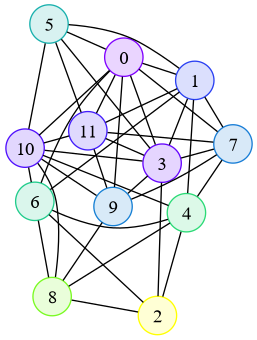
\includegraphics{ex6a.png}

  \newpage
  \item[(b)]
  Color legend:

\colorbox[HTML]{ffff00}{\color[HTML]{ffff00} 000} 4 \\
\colorbox[HTML]{51f242}{\color[HTML]{51f242} 000} 5 \\
\colorbox[HTML]{51f242}{\color[HTML]{51f242} 000} 5 \\
\colorbox[HTML]{17afaf}{\color[HTML]{17afaf} 000} 6 \\
\colorbox[HTML]{17afaf}{\color[HTML]{17afaf} 000} 6 \\
\colorbox[HTML]{17afaf}{\color[HTML]{17afaf} 000} 6 \\
\colorbox[HTML]{17afaf}{\color[HTML]{17afaf} 000} 6 \\
\colorbox[HTML]{2942f2}{\color[HTML]{2942f2} 000} 7 \\
\colorbox[HTML]{2942f2}{\color[HTML]{2942f2} 000} 7 \\
\colorbox[HTML]{8000ff}{\color[HTML]{8000ff} 000} 8 \\
\colorbox[HTML]{8000ff}{\color[HTML]{8000ff} 000} 8 \\
\colorbox[HTML]{8000ff}{\color[HTML]{8000ff} 000} 8

  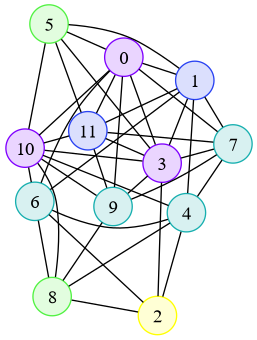
\includegraphics{ex6b.png}
\end{enumerate}

\end{document}
